\section{Simulation of the controller}
 To simulate the the block diagram of p controller with the kp value calculated and the transfer function of the z-axis matlab Simulink is used. The block diagram in figure \ref{fig:Mat_Lab} simulate the behaviour of the system, when flying the drone in z-axis. 
 \begin{figure}[H]
     \centering
     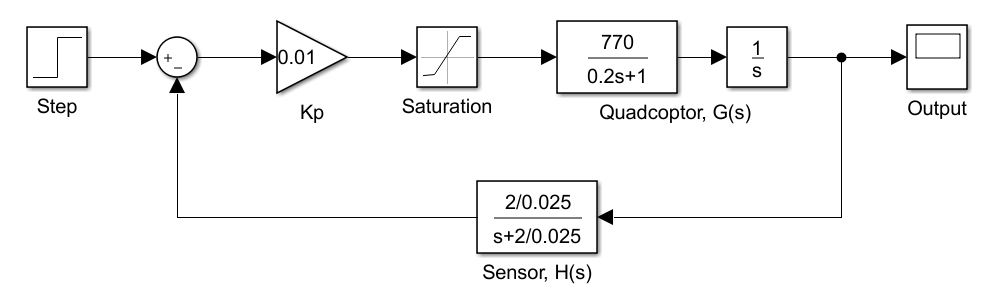
\includegraphics[width=\textwidth]{figures/ch_movement/matlab_block.png}
     \caption{Block diagram.}
     \label{fig:Mat_Lab}
 \end{figure}
By using the simulink the output of the block diagram which is the step response in this case be simulated as shown on figure \ref{fig:simu}. The step response can be used as a verification tool to check if the system meets the specifications from the requirement specification. 
\begin{figure}[H]
    \centering
    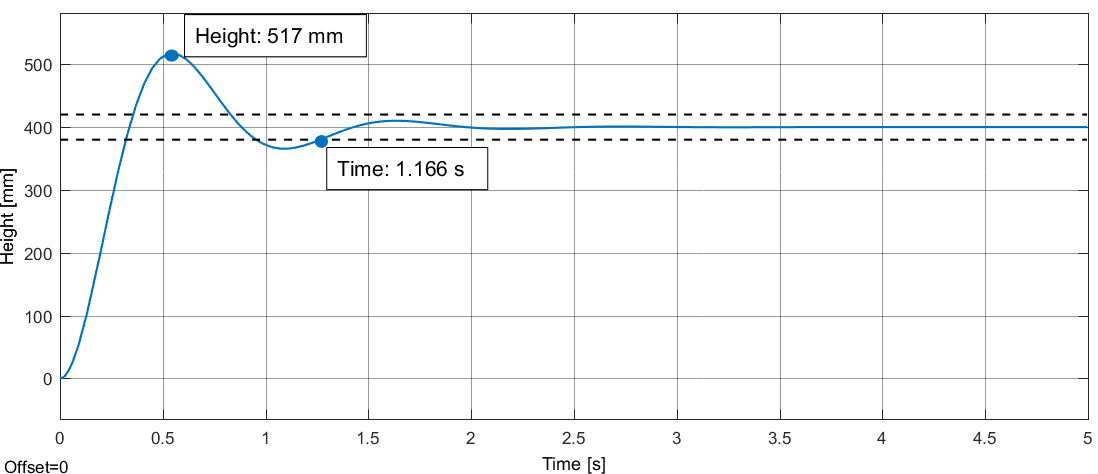
\includegraphics[width=1\textwidth]{figures/ch_movement/Simu.png}
    \caption{Simulation of the output from the block diagram.}
    \label{fig:simu}
\end{figure}% skal ændres
The settling time is read to 1.166 s, which meets the requirement with a desired settling time of $\leq$10 s.\\
The overshoot can be calculated by using the peak value from the step response with equation \ref{eq:overshoot}.
\begin{equation}\label{eq:overshoot}
   PO=\frac{517-400}{400}\cdot 100 = 29.25\%
\end{equation}
From the simulation of the controller, the system holds the required overshoot at $\leq$30\%. And therefore the designed controller will be used in the project.
